\documentclass[11pt,twoside]{report}
\usepackage{preamble}
\graphicspath{{../img/ch4/}}
\setcounter{chapter}{4}


\begin{document}

\chapter{Observing Zebrafish in 3D}
\label{chapter:fish_3d}

\epigraph{
奇肱之国在其北~其人一臂三目
}{\emph{What is a scientist}}

\section{Introduction}hartley2003

This chapter would present the method to build up a 3D tracking system for the zebrafish, and the results obtained from the custom 3D tracking system. This tracking system is inspired by the pioneering work of \citeauthor{cavagna2008} \cite{cavagna2008} and \citeauthor{kelley2013} \cite{kelley2013}, where the 3D locations of European starlings and midges were calculated. Performing the same task on the fish schools is slightly harder for the refraction of light at the water--air interface, and the way to handle the refraction would be discussed.

To carry out the 3D tracking, it is important to understand the formation of the image on a camera, because one needs to reverse the formation process to get the 3D locations. The formation of images on a camera is identical to the way we perceive the world visually, and it will be covered as a brief introduction of projective geometry in chapter~\ref{chapter:multi_view}. With the mathematical basis of projective transformations, I will introduce the pinhole camera model, including the practical ways to calibrate the cameras. The knowledge of the projective geometry and camera model would enable one to find 3D locations of objects from different 2D images.

However, the real measurements are never perfect. The 2D measurements of the fish positions can be problematic, as described in the previous chapter. In addition, new errors would also emerge from the camera calibration process, as well as the wrong association of identities in different views (different cameras). The errors create ambiguities during the locating of 3D coordinates, and some practical ways to cope with the ambiguities would be discussed in this chapter.

Applying the 3D observation method, I will present the result for the wildtype zebrafish with different group sizes. 


\section{Viewing Fish with Many Eyes}

This section should serve as a practical tutorial for building a multiple view 3D system to track animals. This system is capable of extracting 3D trajectories, with commercial cameras.

It is not the only technology for such task. Instead, there are alternative ways to follow the movement of animals such as binding animals with global positioning system (GPS) \cite{nagy2010} and tagging the animal bodies \cite{jolles2017}. Comparing with these solutions, the system to be introduced is non-invasive and relatively cheap. However, the obtained trajectories were not perfect, due to the errors of the 2D locating of fish individuals (section \ref{section:image_process}), and the ambiguity in the linking process (section \ref{section:link}).

The mathematical basis of this chapter is introduced in appendix~\ref{chapter:multi_view}, and it is necessary to understand the projective transformation and camera models to implement the 3D reconstruction algorithms. Ignoring the tedious details, the section will instead focus on the introduction of the practical 3D tracking apprautus. We should be confident about the way 3D tracking works, and even be able to start our own 3D tracking lab, upon finishing this section.

\subsection{Tank Design and the Hardwares}
\label{section:system_3d}

Figure \ref{fig:lab} shows the experimental setup in the laboratory, where I mounted 3 cameras pointing to a bowl--shaped tank. This big bowl was immersed in a framed swimming pool, and the swimming pool was covered with plastic balls\marginfootnote{Curiously, immersing plastic balls inside the fish tank is also something physicists do to explore the structure of the simple liquid in 1930s. \cite{travis2021}} to reduce the evaporation of water. Synchronised signals were generated with a Arduino chip, and the cameras are able to capture time--synchronised videos with the signals. The trigger signal for the camera is a 5V pulse, being the default \texttt{HIGH} output signal of an Arduino chip.


The big, white plastic bowl was specially designed and manufactured to contain the fish. The choice of the shape was based on the fact that the fish tend to stay in the corner of the tank, when they entered an unfamiliar environment. Using a bowl--shaped container prevented the aggregation at the corners. Except for the corner effect, the bowl also provides no blind zone for all of the cameras, preventing the systematic disappear and reappearing of the fish in the video.


The zebrafish are living animals, and it is also important to provide them a suitable condition. Typically, the fish need a temperature between 25 \degree C and 30 \degree C, and the water should be constantly filtered and sterilisation with UV light. All of the related equipments re placed outside the bowl--shaped tank, but inside the swimming pool, so that they would not affect the behaviours of the fish. Knowing the boundary, it allows us to calculate excess probabilities distribution functions like the radial distribution function, because it is now possible to generate uniformly distributed random points inside the tank. 


\begin{SCfigure}
  \includegraphics[width=0.8\linewidth,outer]{lab.jpg}
  \caption[Three dimensional fish tracking system]{The photo of one experimental setup. Three cameras were mounted to observe the fish in the bowl shaped tank. Time--synchronised signals were generated by a Arduino chip to trigger the cameras for capturing synchronised videos. The bowl was immersed in a bigger tank, which is a framed swimming pool. The husbandry--related equipments, such as the water filter, the heaters, the UV lamp, were placed outside the bowl but inside the bigger tank.}
  \label{fig:lab}
\end{SCfigure}


I also measured the 3D shape of the tank to know the exact boundary for the fish. The measurement was performed by placing markers on the surface of the tank, and then reconstruct the markers in 3D. Since the tank is rotationally symmetric around the z--axis, it is appropriate to describe its geometry in the cylindrical coordination system with the hight ($z$) and the radius ($r$). Figure \ref{fig:tank} shows the results of the measurement, and the shape of the tank can be modelled by function $z=0.734 r^2$, where both length variables take the units of meter. The shape of the tank, together with the water level, are the boundaries for the movement of the fish.

\begin{SCfigure}
  \includegraphics[width=0.5\linewidth]{tank-fit.pdf}
  \caption[The 3D geometry of the observation tank.]{The measured shape of the observation tank. The scatters were markers on the tank, which were fitted by function $z=0.734 r^2$, where the unit of both $z$ and $r$ is meter.}
  \label{fig:tank}
\end{SCfigure}



\subsection{Handling the Refraction}
\label{section:refraction}


\subsection{Locating Fish in 3D}
\label{section:locate_3d}

The task of finding the 3D positions of zebrafish consists of two parts. The first part is finding the positions of fish in individual views, and the method is discussed in the previous chapter. The second part is to integrating the positions from different views and the knowledge of about the cameras, to calculate the 3D locations.


\begin{SCfigure}
  \includegraphics[width=0.8\linewidth]{track-3d-idea}
  \caption[Three dimensional tracking concept illustration]{Tracking the fish with three cameras. This figure demonstrates the idea of obtaining the 2D locations of fish with the input of 1D information. Each inserted box shows the projection of the fish onto the camera. Knowing the location of the centres of the cameras, one can re-cast the rays responsible for the projection of the fish. The intersections of the re-casted rays are the locations of the fish.}
  \label{fig:track_idea_3d}
\end{SCfigure}

\subsection{Refine the Trajectories}

The 3D positions obtained from the tracking system can be linked into trajectories described in section \ref{section:link}. The linked trajectories are good, thanks to the predictive linking method and the subsequent relinking, but it is still possible to further optimise the trajectories. The idea is to re--incorporate the information of the 2D features and cameras into the trajectories.

\subsection{The Accuracy of the Method}

I evaluated the accuracy of the tracking method with the simulated data. Typically, I generated the trajectories of 50 simulated fish inside a container. Then I use the software \emph{Blender} (version 2.91.0 on Ubuntu 20.04) to render the movement of the fish as animations, with multiple cameras. The result movies looks very similar to my experimental videos, in terms of the local fish density and the speed. This similarity ensured the accuracy that I assessed from the simulation movie is valid for my experimental data.


\section{The 3D Spatial Distribution of Zebrafish}

The 3D tracking yields the positions of the fish, whose discrete time derivative gives the velocities. From these two quantities, we calculate three global descriptors to characterise the behaviour of the fish: the average speed, the polarisation, and the nearest neighbour distance. The average speed is defined as $v_0 = 1/N \sum{|\vi|}$ where $i$ runs over all the tracked individuals. 

For experiments with more than one fish, the polarisation $\Phi$ was commonly used to characterises the alignment of the velocities. It is defined as the modulus of the average orientation, written as \cite{attanasi2014pcb},
$\Phi = 1/N \left| \sum{({\vi}/{| \vi |}}) \right|$ where $i$ runs over all the individuals. Large polarisation ($\Phi \sim 1$) signifies synchronised and ordered movement, while low polarisation indicates decorrelated, random movement. The polarisation is sometimes referred to as the ``order parameter'' by physicists, since it is a measure of the order of the fish dynamic. We say a group of fish have \emph{ordered} movement if they are swimming towards the same direction.\marginfootnote{If we think of the moving direction of the fish as little spins of a magnetic system, then the polarisation is mathematically equivalent to the average magnitisation per spin.}

The local density of the group also plays important roles in the collective behaviour. The local density can be probed by the nearest neighbour distance, which is noted as {\dnn} in this thesis. For a fixed number ($N$) of fish in a fixed sized environment (with volume $V$), their overall number density is constant (being $N/V$). However, the groups with smaller {\dnn} is more cohesive.


\subsection{A Single Fish}
\label{section:fish_1_3d}


Figure~\ref{fig:density_3d_fish_1} shows the spatial distribution of one fish in the observation tank. It is obvious that the fish tend to stay in the bottom of the tank. It is a typical fish behaviour when they were subjected to a new environment, and it is known as the ``depth preference''.
Nevertheless, the distribution of the $X$ components of the coordinates is symmetric, which suggests the fish do not have a preferred location to stay in the tank.


\begin{SCfigure}
  \includegraphics[width=\linewidth,outer]{density-one-fish}
  \caption[The 3D spatial distribution of one fish]{The spatial distribution of one adult zebrafish. The top panel shows the joint distribution of the $Y$ coordinates and $Z$ coordinates of the fish positions. The bottom panel shows the distributions of the $X$ coordinates, the planar radius ($R$) and the $Z$ coordinates. The distribution of the ideal gas in the tank was given as a reference.}
  \label{fig:density_3d_fish_1}
\end{SCfigure}

From the fish trajectories, we can also calculate their speed and orientations in each from. These time series also offer the typical time scale of speed changing and orientation relaxing.


\subsection{A Pair of Fish}
\label{section:fish_2_3d}

The spatial distribution of 2 zebrafish were presented in Fig~\ref{fig:density_3d_fish_2}. The behaviour of 2 fish is similar to that of one fish. Namely, the fish tend to be around the bottom of the tank.

\begin{SCfigure}
  \includegraphics[width=\linewidth,outer]{density-two-fish}
  \caption[The 3D spatial distribution of two fish]{The spatial distribution of two adult zebrafish. The top panel shows the joint distribution of the $Y$ coordinates and $Z$ coordinates of the fish positions. The bottom panel shows the distributions of the $X$ coordinates, the planar radius ($R$) and the $Z$ coordinates. The distribution of the ideal gas in the tank was given as a reference.}
  \label{fig:density_3d_fish_2}
\end{SCfigure}

The fish interaction can be probed by the relative distribution of the neighbours of the fish. 


\subsection{Three Fish}
\label{section:fish_3_3d}

The spatial distribution of 2 zebrafish were presented in Fig~\ref{fig:density_3d_fish_3}. Being similar to the one fish and two-fish case, a group of three fish presents the depth preference.

\begin{SCfigure}
  \includegraphics[width=\linewidth,outer]{density-three-fish}
  \caption[The 3D spatial distribution of three fish]{The spatial distribution of three adult zebrafish. The top panel shows the joint distribution of the $Y$ coordinates and $Z$ coordinates of the fish positions. The bottom panel shows the distributions of the $X$ coordinates, the planar radius ($R$) and the $Z$ coordinates. The distribution of the ideal gas in the tank was given as a reference.}
  \label{fig:density_3d_fish_3}
\end{SCfigure}

\subsection{Many Fish}
\label{section:fish_many_3d}

We studied the behaviour of 50 fish with two different age groups, the {\smallfish} whose age is between 6 months old to 1 year, and the {\bigfish} whose age is beyond 1 year.

The behavioural quantities, as I summarised in Table~1, is shown in Fig~\ref{fig:descriptor-many-fish}.

\begin{SCfigure}
  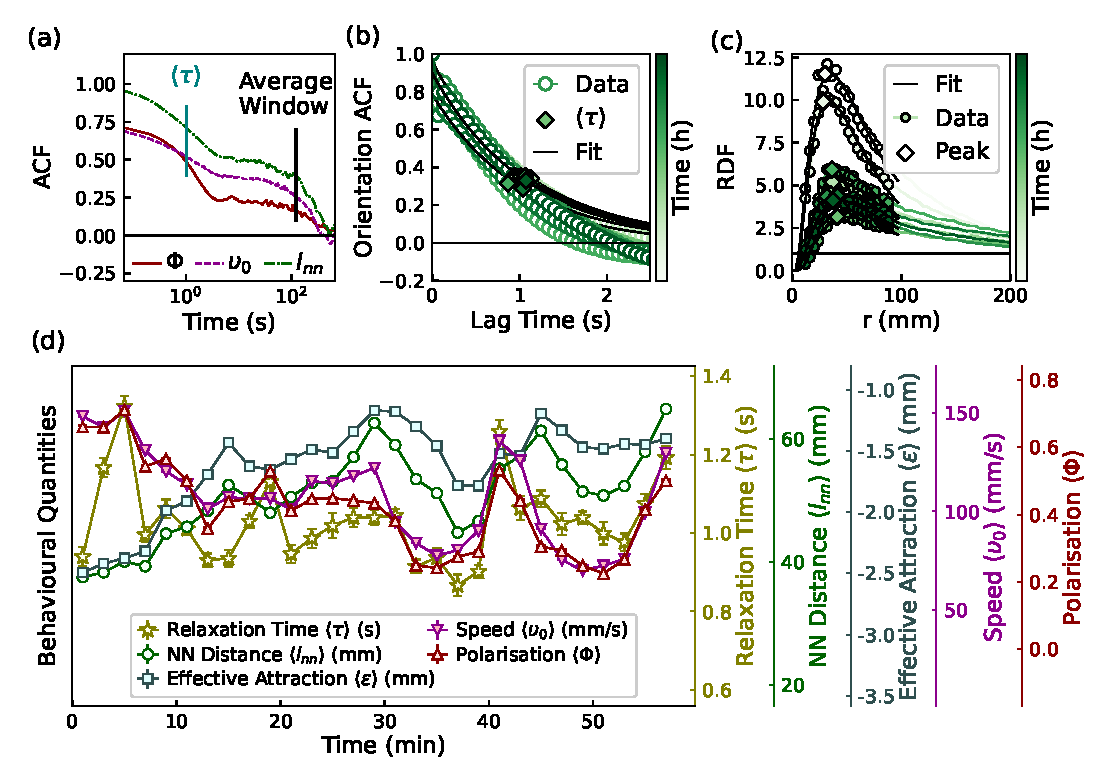
\includegraphics[width=\linewidth,outer]{descriptor-many-fish}
  \caption[The behavioural descriptors of 50 zebrafish]{
  	(a): The auto--correlation function of the polarisation and average speed of the fish group.
	(b): The auto--correlation function of the orientations of fish.
	(c): Sequence of radial distribution functions with increasing time: at early times (top curves) the fish are clustered together so that the peak is large; at later times (bottom curves) the local density decreases and so does the peak height.
	(d): The time evolution of the averaged {\descriptors} for 50 {\smallfish} fish. Each point corresponds to the average value in 2 minutes.
	The error bars illustrate the standard error values.
  }
  \label{fig:descriptor-many-fish}
\end{SCfigure}

\section{Conclusion}

\end{document}
